%
% teil3.tex -- Beispiel-File für Teil 3
%
% (c) 2020 Prof Dr Andreas Müller, Hochschule Rapperswil
%
% !TEX root = ../../buch.tex
% !TEX encoding = UTF-8
%
\subsection{Mutation
\label{genetic_algorithm:mutation}}
Dieser Schritt ist dafür da da sich zufällige änderungen in den 
Genen stattfindet. Dies soll dazu führen, dass neue Gene entstehen, 
wodurch der gesammte Lösungsraum grösser wird. Es sollte so 
verhindert werden, dass plötzlich nur noch die gleichen 
Genmuster entstehen sondern auch etwas neues enstehen kann. 
Ein guten Vergleich zu maschinelles Lernen wäre es, dass man so 
versucht aus einem Extrempunkt herauskommen.

Würde der genetischer String nur aus 0 und 1 bestehen. Würden zufällig 
Stellen einfach ein und ausgeschaltet. Dies ist daher mit den Stätten 
auch nicht möglich, daher werden Teile mit einander vertauscht.

\begin{figure} [h]
	\centering
	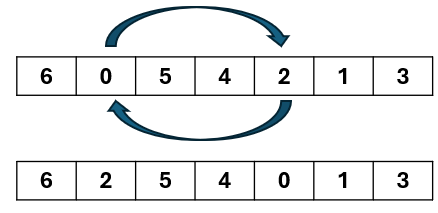
\includegraphics[width=0.8\textwidth]{
        papers/variationsprinzip_algorithmen/images/teil3/09_genetic_string_cities_mutation.png
        }
	\caption{Beispiel einer Mutation}
	\label{fig:mutation_genetic_string}
\end{figure}

Der Teil besitzt auch keine Mathematische Formel, es geht einfach um die 
Logik welche 2 zufällig Stellen nimmt, diese Tauscht um eine neue 
Variation von Lösungen zu erstellen. Welche bei der Kreuzung nicht enstanden
wäre.
